% import
\documentclass[conference]{IEEEtran}
\IEEEoverridecommandlockouts
\usepackage{cite}
\usepackage{amsmath,amssymb,amsfonts}
\usepackage{algorithmic}
\usepackage{graphicx}
\usepackage{textcomp}
\usepackage{xcolor}
\usepackage{diagbox}
\usepackage{hyperref}
\usepackage{color, colortbl}
\usepackage{multirow}
\def\BibTeX{
    {\rm B\kern-.05em{
        \sc i\kern-.025em b
    }\kern-.08em T\kern-.1667em\lower.7ex\hbox{E}\kern-.125emX}
}

% url & cite styling
\hypersetup{
    colorlinks=true,
    citecolor=black,
    urlcolor=cyan,
    linkcolor=black
}

% color definition
\definecolor{moreratio}{rgb}{0,1,0}
\definecolor{lessratio}{rgb}{0.95,0.5,0.5}
\definecolor{tableheader}{rgb}{0.8,0.8,0.8}

% document start
\begin{document}

\title{Searching Algorithm for Match Mapping in Kidney Exchange Program}

% author
\author{\IEEEauthorblockN{Fazat Nur Azizah}
\IEEEauthorblockA{fazat@informatika.org}
\and
\IEEEauthorblockN{Ardian Umam}
\IEEEauthorblockA{ardian@informatika.org}
\and
\IEEEauthorblockN{Leonardo}
\IEEEauthorblockA{leonardow41@gmail.com}
}

\maketitle

\begin{abstract}
Before kidney transplant is performed, the kidney donor and the kidney recipient must
be a compatible pair. In reality, it's not uncommon that incompatibility occurs between the donor-recipient pair.
To solve this problem, Kidney Exchange Program was created so that an incompatible pair can exchange the kidney
to another incompatible pair, making cross donation easier. But to search for the optimal match map from incompatible
pairs pool is not an easy task. Match map searching algorithm is an algorithm created for this task. Edmond's
Algorithm, the existing algorithm, is suboptimal because it closes the possibiliy of three or more-way exchanges.
Therefore, in this paper, by modifying existing two-way match map searching algorithms, \textit{N}-way match
map searching algorithm is implemented. Based on the test results, using 3000 incompatible pairs data, it is
proven that \textit{N}-way match map searching algorithm is superior in terms of matching efficiency compared to
the two-way match map searching algorithm. The increase in matching efficiency obtained on average reaches 7.75\%
in comparison to the matching efficiency obtained by Edmond's Algorithm. 
\end{abstract}

\begin{IEEEkeywords}
kidney transplantation, kidney exchange, match map searching algorithm
\end{IEEEkeywords}

\section{Introduction}
Kidney transplantation is the most recommended treatment method for serious kidney diseases \cite{roth2005}.
Every year, in Indonesia alone, there are more than 100,000 patients with kidney transplantation needs. But among
those patients, only about 20\% can get a kidney transplantation \cite{wiradarma}. There are many types
of problems that leads to this condition, for example financial problems, public opinions, and the most
common, kidney availability.
Even though live donor numbers are steadily increasing\cite{roth2006}, availability problem arises because many criteria must
be met before kidney transplant can be performed \cite{wiradarma}. The donor needs to have a healthy kidney,
matching blood type, and no blood-borne diseases. Also, the patient's immune system must be able to accept
the donor's kidney without killing it.

\subsection{Kidney Transplant Prerequisites}
\begin{table}[htbp]
    \caption{Blood Type Compatibility between Patient and Donor \cite{raja}}
    \begin{center}
    \def\arraystretch{1.5}
    \begin{tabular}{|c|c|c|c|c|}
    \hline
    \cellcolor{tableheader}\backslashbox{\textbf{Recipient}}{\textbf{Donor}}&\cellcolor{tableheader}\textbf{O}&\cellcolor{tableheader}\textbf{A}&\cellcolor{tableheader}\textbf{B}&\cellcolor{tableheader}\textbf{AB} \\
    \hline
    \cellcolor{tableheader}\textbf{O}&1&0&0&0 \\
    \hline
    \cellcolor{tableheader}\textbf{A}&1&1&0&0 \\
    \hline
    \cellcolor{tableheader}\textbf{B}&1&0&1&0 \\
    \hline
    \cellcolor{tableheader}\textbf{AB}&1&1&1&1 \\
    \hline
    \end{tabular}
    \label{tab1}
    \end{center}
\end{table}

There are few tests that have to be performed before kidney transplant can be done \cite{adrian}.
The blood type test is performed to both the donor and the recipient. Donors can only make a
donation if one's blood type is compatible with the recipient's blood type.
In Table I, number 1 indicates compatibility and 0 indicates incompatibility. Donors with blood type
O are considered Universal Donors because they can give donors to every patients regardless of the blood
type. Recipients with blood type AB are considered a Universal Recipients because they can accept kidney
donation from every donors regardless of the blood type \cite{charge}.
The immune test is performed after the donor-recipient pair passes the blood type test \cite{adrian}. The tests
are cross match test and Human Leucocyte Antigen (HLA) test. In cross match test, donor's blood are met with
recipient's blood to see whether there is a resistance reaction from recipient's immune system. The resistance
reaction happens when the donor kidney is considered a foreign object that must be killed by recipient's
immune system \cite{aprilano}. HLA test tests the same reaction as cross match test, but donor's and recipient's
tissue cells are being used instead of blood \cite{nguyen}.
Finally, to test whether the donor has any blood-borne diseases, serology is performed \cite{aprilano}.

\subsection{Kidney Exchange Program}
Because of kidney transplant prerequisites, Kidney Exchange program named Kidney Paired Donation (KPD) was created
so that an incompatible donor-recipient pair can exchange their incompatible kidney to another incompatible
pair, making cross-donation possible \cite{raja}. The kidney exchange can be done two-way, three-way, and can
go up to \textit{N}-way.

\begin{figure}[h]
    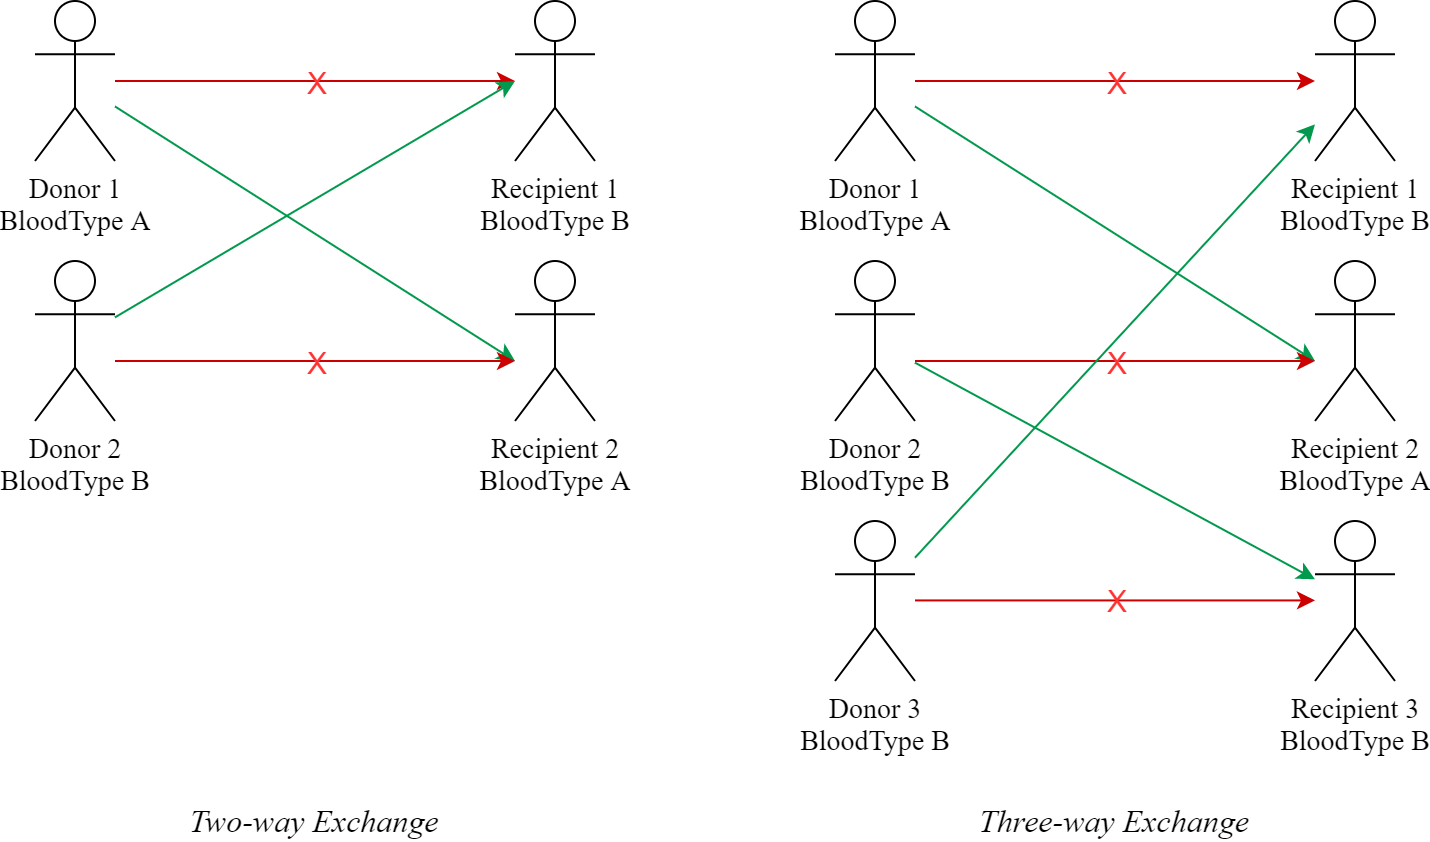
\includegraphics[width=0.5\textwidth]{images/kidney-exchange.png}
    \caption{Two-way(left) and Three-way(right) Exchange in KPD program}
\end{figure}

Unfortunately, because of the large number of incompatible pairs, hospitals cannot find the optimal
matching solution for the pool of incompatible pairs. An algorithm that perform a mapping search is needed
to address this issue. One of the most known algorithm to tackle this problem is Edmond's Algorithm \cite{raja}.
In Edmond's Algorithm, the pool of incompatible pairs are represented as a graph with each node representing
an incompatible pair and each edge representing a match between two incompatible pairs. The algorithm focuses on
high priority pairs so that pairs who need a transplantation more can get an exchange first.
Another algorithm regarding this problem is First Accept Heuristic Match \cite{raja} which focuses more on the
heuristic if one registers first, then one gets an exchange first.

These algorithms are called Match Map Searching Algorithms. To evaluate and measure the performance of an algorithm,
a few specific performance metrics are use\cite{tullis}. There are two performance metrics to evaluate these
algorithms. The first one is Matching Efficiency, which measures the number of donor-patient pairs that matched
another pair and were able to exchange divided by the total number of donor-patient pairs, represented in a percentage.
The second metric is execution time, which measures how long does the algorithm run to get the optimal match map,
usually measured in millisecond. The best match map searching algorithm is the algorithm that can produce high matching
efficiency with low execution time. Meaning that many patients can be saved as fast as possible.

As good as it looks, Edmond's Algorithm and First Accept Heuristic Match can only find two-way exchanges from the
incompatible pairs pool. Meaning these algorithms are not able find a solution with three-way exchanges or more,
closing the possibility.

\section{Methodology}
From the existing algorithms problems addressed in the previous section, match map searching algorithms that can find
\textit{N}-way exchanges from incompatible pairs pool are needed. By modifying existing algorithms and the used data
structure, new algorithms can be created.

\subsection{Modifications for Existing Algorithms}
Before creating new algorithms, incompatibility pairs pool data structure needs to be redefined. Compatibility Graph
used in Edmond's Algorithm is an undirected graph \cite{raja}, meaning that every edge connecting two vertices represent a bidirectional
relationship between the aforementioned two vertices. Therefore the exchanges can be detected by getting the edges of the
compatibility graph, closing up possibility of three-way exchanges or more. If the algorithm is modified to use cycle detection
instead of edge detection, Edmond's Algorithm can already be used to return \textit{N}-way exchanges.
As seen in Fig. \ref{edgevscycle}, using cycle detection yields a result with three-way exchange instead of the two-way exchange result
returned by edge detection, resulting in a higher matching efficiency using the same compatibility graph. 

\begin{figure}[h]
    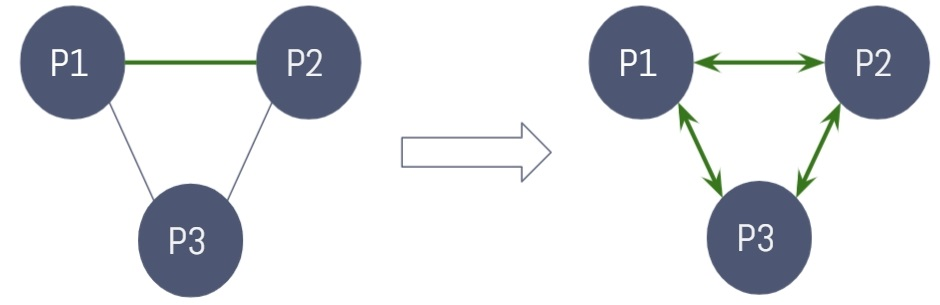
\includegraphics[width=0.5\textwidth]{images/edge-vs-cycle-detection.jpg}
    \caption{Edge Detection(left) vs. Cycle Detection(right) in Compatibility Graph}
    \label{edgevscycle}
\end{figure}

Edge detection used in existing algorithms needs to be converted to cycle detection to increase matching efficiency.
However, changing edge detection to cycle detection is not enough. The cycles returned from the graph are all bidirectional
cycles. If the compatibility graph is converted into a directed graph instead of undirected, unidirectional cycles can also be
returned, further increasing the number of cycles, therefore increasing the matching efficiency as seen in Fig. \ref{undirectedvsdirected}.
Directed graph is a data structure consisting a set of vertices that are connected via edges, where each edge has a one-way
direction that shows the direction of movement from one vertex to another \cite{sedgewick}.
Cycle detection for directed graph is used to find the existence of a one-way path in a graph that starts and finishes
at the same vertex \cite{mehta}.

\begin{figure}[h]
    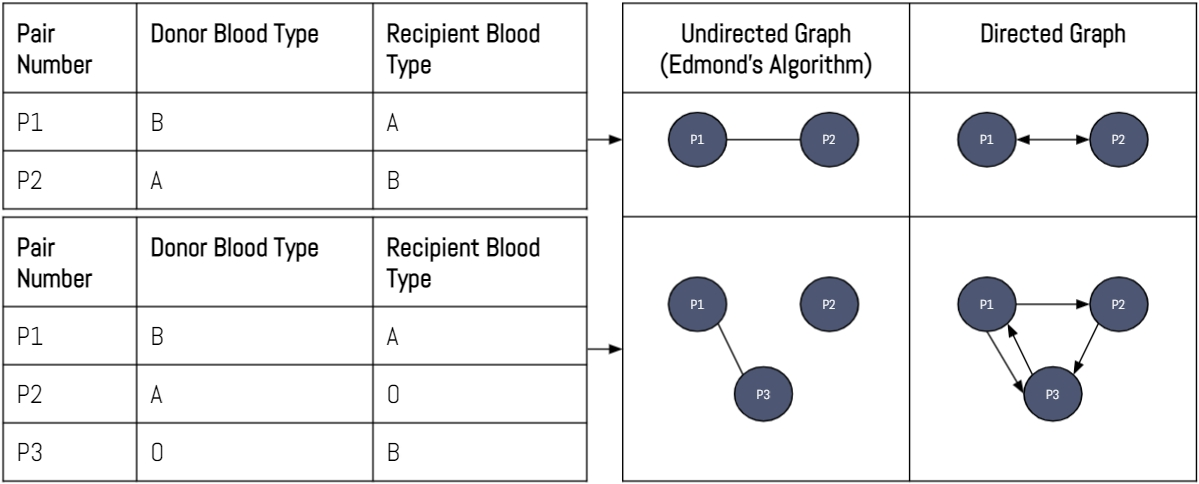
\includegraphics[width=0.5\textwidth]{images/undirected-vs-directed-compatibility-graph.jpg}
    \caption{Undirected vs. Directed Compatibility Graph}
    \label{undirectedvsdirected}
\end{figure}

The cycle detection algorithm being used here is a little bit different from the usual cycle detection algorithm that detects
whether a graph has a cycle or not, instead this algorithm collects and returns all possible cycle in a graph in a list.
Each cycle in this list is a possible exchange that can be excecuted. The length of the cycle represents the \textit{N} in
\textit{N}-way exchange (e.g., a cycle with the length of 3 represents a three-way exchange).
These modification is performed with the hope that the amount of cycles being detected will
increase and therefore increasing matching efficiency and saving more patients.

\subsection{\textit{N}-way Match Map Searching Algorithms}
With directed graph as compatibility graph and using cycle detection algorithm, \textit{N}-way match map searching algorithms
can be created. This algorithms receive the list of cycles returned from cycle detection and returned a reduced list of cycles
called match mapping. The reduction mentioned is done because each pairs in compatibility graph can exist in more than one cycles
in list of cycle, creating a many-to-many relationship among the pairs. This is obviously impossible as every pair can only donate
and receive exactly one kidney. The reduction is done to change this many-to-many relationship to be a one-to-one relationship. This
reduction usually leaves some pairs to be not matched at all, therefore matching efficiency is used as a performance metric to
measure how many pairs can get matched out of the full incompatible pairs pool.  

\subsubsection{First Accept Searching Algorithm}
The first \textit{N}-way match map searching algorithm is first accept searching algorithm which is inspired by first accept
heuristic match algorithm. The first-accept approach being used in this algorithm is to to use the first cycles in cycles list
returned from cycle detection algorithm. This algorithm ensures that no pair gets matched twice or more by deleting cycles that
contains pairs that have been matched earlier.

This algorithm uses two parameters. The first parameter is the number of \textit{N}, knowing that this algorithm is an \textit{N}-way
algorithm. The second parameter is the method to use \textit{N}. The number of \textit{N} can be used as a maximum or exact way of exchanges.
When the maximum method is used, the algorithm will search for cycles that represents two-to-\textit{N}-way exchanges. Meanwhile when exact
method is used, the algorithm will search for cycles that have an exact length of \textit{N}.

Even though maximum method blindly looks like a certainly superior method than exact method, it is not always the case. For example, as can be
seen in Fig. \ref{maxvsexact}, when \textit{N} is 5, when maximum method is used, the bidirectional cycles in compatibility graph is
returned first, removing the five-way exchange possibility. When exact method is used, the bidirectional cycles is not returned because
the algorithm only looks for five-way exchanges, therefore returning the five-way exchange. In this case, higher matching efficiency
is achieved when exact method is used instead of maximum method.

\begin{figure}[h]
    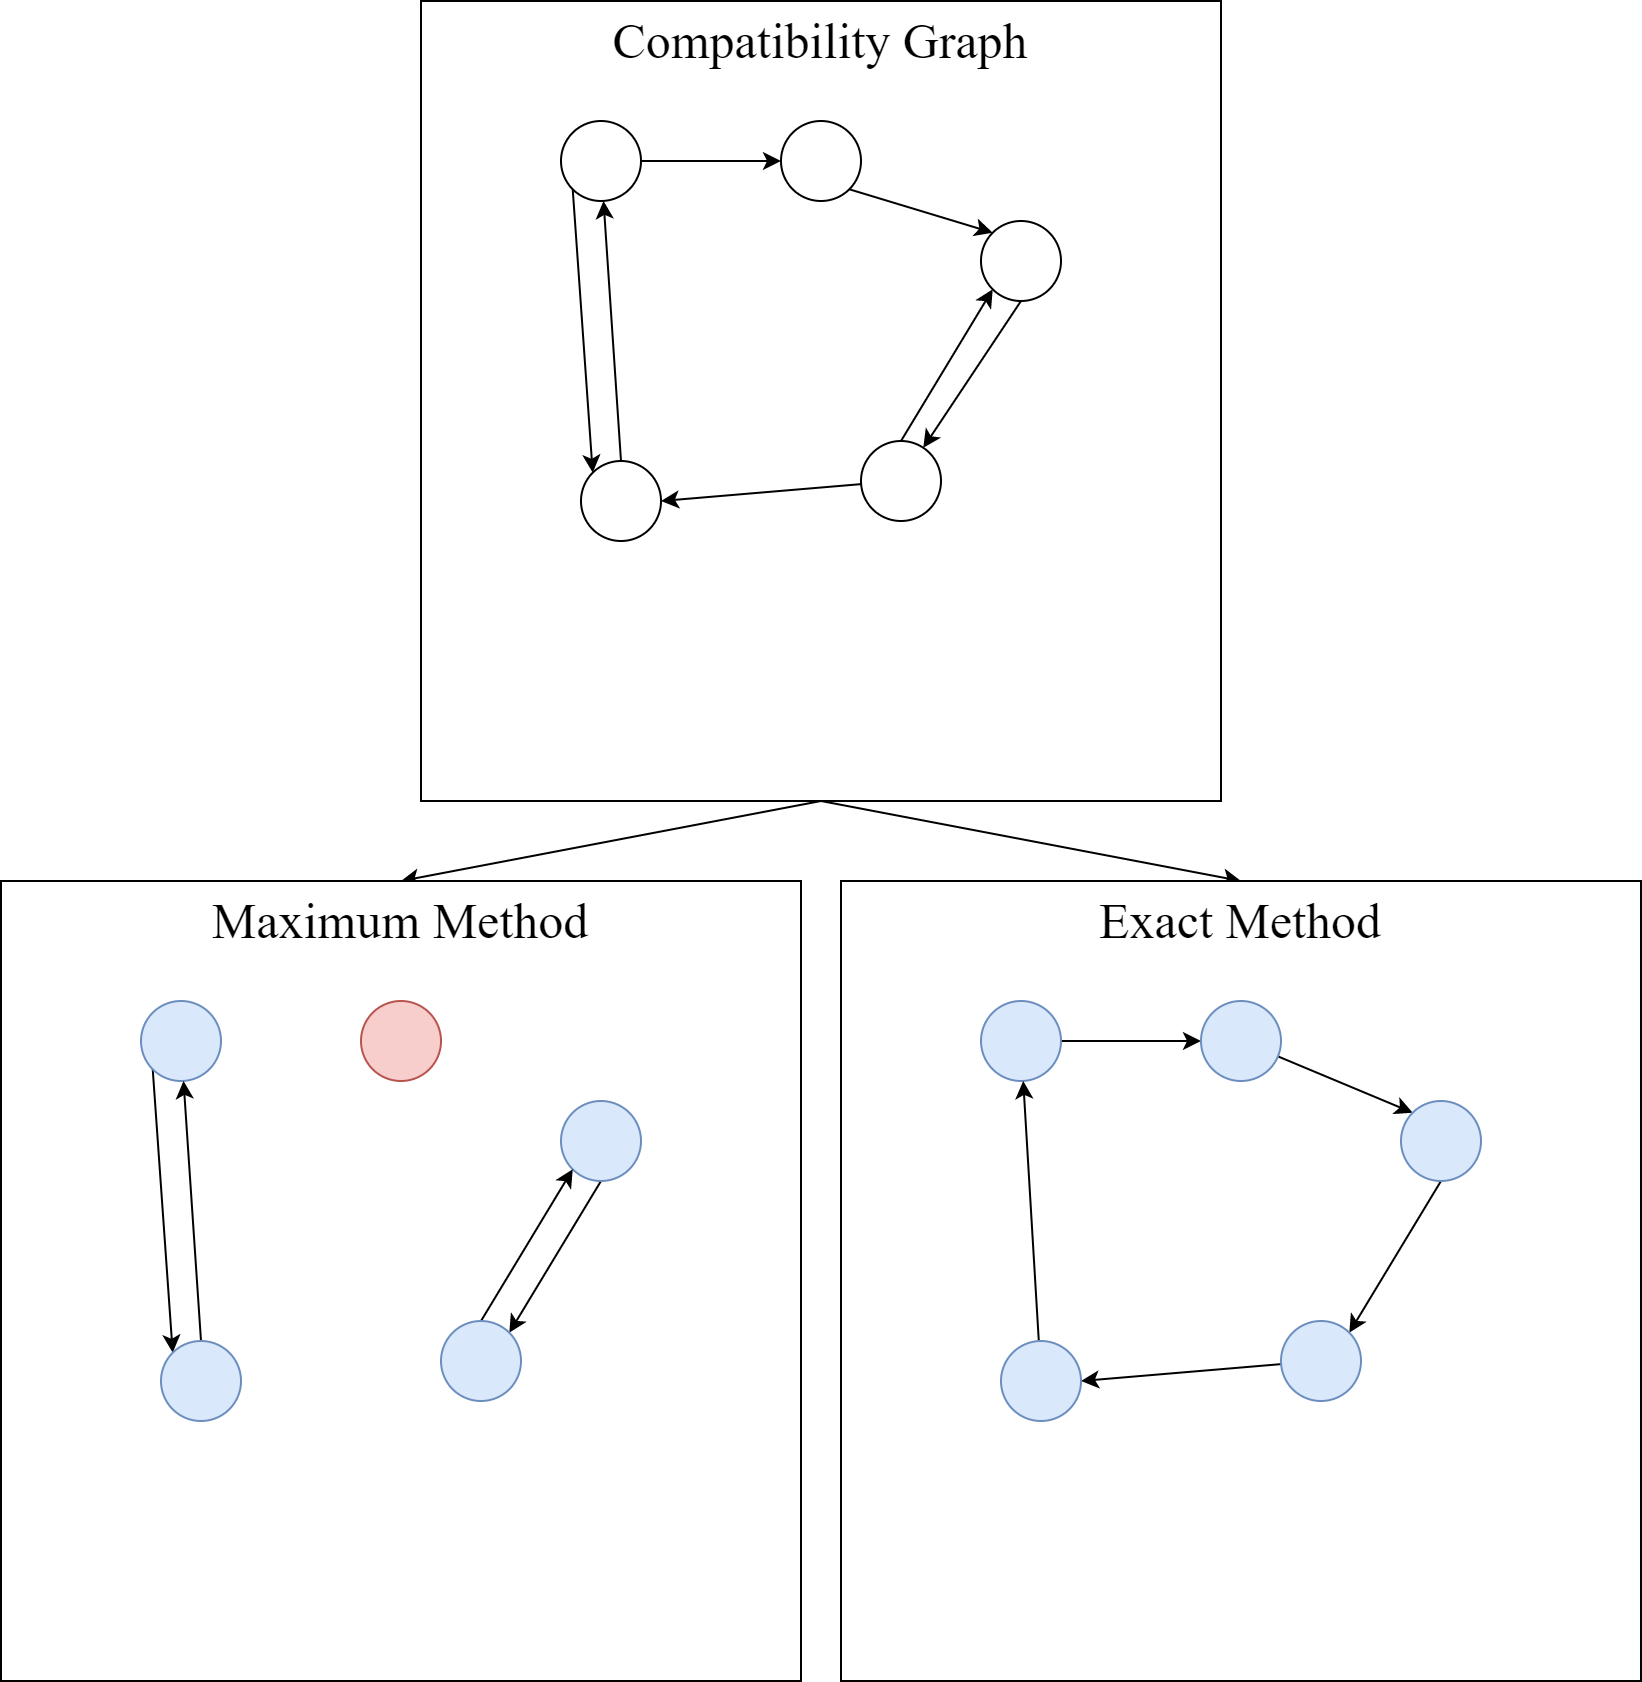
\includegraphics[width=0.5\textwidth]{images/maximum-vs-exact.png}
    \caption{Case where Exact Method is superior to Maximum Method}
    \label{maxvsexact}
\end{figure}

\subsubsection{Priority-based Searching Algorithm}
The second \textit{N}-way match map searching algorithm is priority-based searching algorithm which is inspired by Edmond's
algorithm. This algorithm works similarly with First Accept Searching Algorithm, but each cycle is given a priority value so
that exchanges with highest priority can be returned first compared to the others.

This algorithm uses three parameters. The first two are the same parameter used in First Accept Searching Algortihm, number of \textit{N}
and the method to use \textit{N}. The third parameter is priority assignment method. There are two methods to measure priority of every cycles.
The first assignment method is the greedy method. This method assigns higher priority for longer cycles, indirectly affecting the algorithm
to return more of the longer cycles with the hope that it can increase the matching efficiency.
The second assignment method is the infrequent method. This method assigns higher priority for cycles with infrequent pairs. In implementation,
infrequent pairs are indicated as vertices that are connected with a low number of edges, meaning that the pairs can only be matched with a low
number of other incompatible pairs.

\section{Experiment and Analysis}
Before experiment is performed, Edmond's Algorithm is also implemented as a baseline algorithm so comparisons can be made against
an existing algorithm. The data being used in this experiment can be found in this link: \url{https://rdm.inesctec.pt/dataset/ii-2020-001}
while the source code of the implementation and the experiment can be found in this link: \url{https://github.com/Mingtaros/Kidney-Exchange-Match-Mapping-System}.
The purpose of these experiments and evaluations are to find the algorithm and parameter combinations which can produce the best
performance results based on pre-defined metrics. In addition, through the experiments, it can be concluded which \textit{N}-way
algorithm and parameter combinations are able to outperform the baseline, Edmond's Algorithm. Based on the pre-defined metrics,
there will be comparison for Execution Time and Matching Efficiency for each algorithm.

\subsection{Execution Time Comparison}
\subsubsection{Execution Time Comparison for Different Algorithm Combinations}
For this experiment, each algorithm is used for 3000 incompatible pairs divided into 30 groups of 100. A group is called a seed. Each
algorithm will be fitted with the same dataset group 50 times for every group. As seen in Figure \ref{exctimealgo}, each data point in the boxplot
is used to show the average execution time from the 50 executions for every dataset group, in one Y coordinate, there are 30 data
points, each one for one data group. 

\begin{figure}[h]
    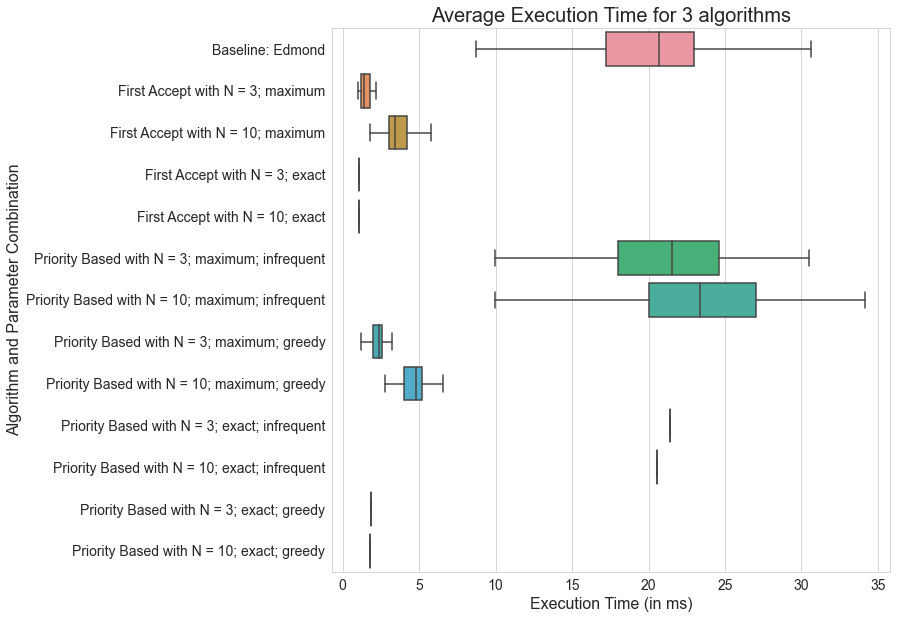
\includegraphics[width=0.5\textwidth]{images/average_execution_time_for_3_algorithms.png}
    \caption{Average Execution Time for 3 Algorithms}
    \label{exctimealgo}
\end{figure}

As seen from the boxplot, Edmond's Algorithm and Priority-based with infrequent method of priority assignment are the slowest
algorithms. However, given that each and every algorithm does not have a significant difference in execution time, the execution
time difference can be ignored.

\subsubsection{Execution Time Comparison for Different Data Sizes}
This experiment is conducted to show the effect of data size to execution time of the match map searching algorithms. For this
experiment, the recorded execution time is the average execution time for each algorithm using data size of  100, 200, 300, 400,
500, 1000, 2000, as well as 3000 incompatible pairs. Each data point is the average of algorithm execution time that has been
executed 10 times for each algorithm for each data size.

\begin{figure}[h]
    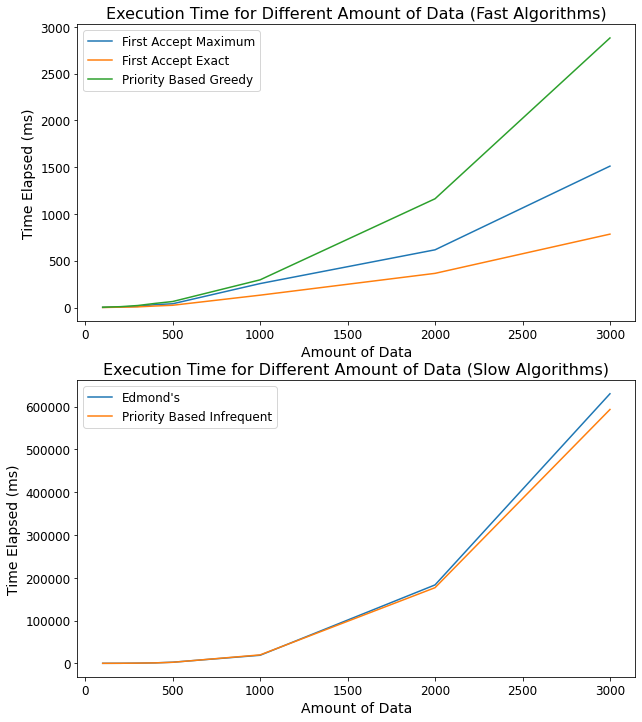
\includegraphics[width=0.5\textwidth]{images/execution_time_for_different_amount_of_data.png}
    \caption{Execution Time for Different Amount of Data}
    \label{exctimedata}
\end{figure}

As seen in Figure \ref{exctimedata}, there are two plots, each one representing a group of fast algorithms and a group of slow algorithms.
From the upper figure, even with 3000 incompatible pairs, the maximum algorithm runtime is around 3000 milliseconds. Meanwhile,
from the lower figure, both of the algorithms can reach 600000 milliseconds (10 minutes) to process 3000 pairs. From the
overall line plot, it can be concluded that the relation of data size and execution time is a form of polynomial function, not linear.

\subsection{Overall Matching Efficiency Comparison for Different Algorithms}
The final experiment is conducted to show which algorithm-parameter combination is the best one in producing high matching efficiency.
In this experiment, each combination is used for every data seed. To ease up the comparison, in Figure \ref{matcheffratio}, ratio of improvement is used
in comparison to Edmond's Algorithm as a baseline shown as a horizontal line in the figure. Every data point is a matching efficiency
multiplier of the matching efficiency obtained when Edmond's Algorithm is used.

\begin{figure}[h]
    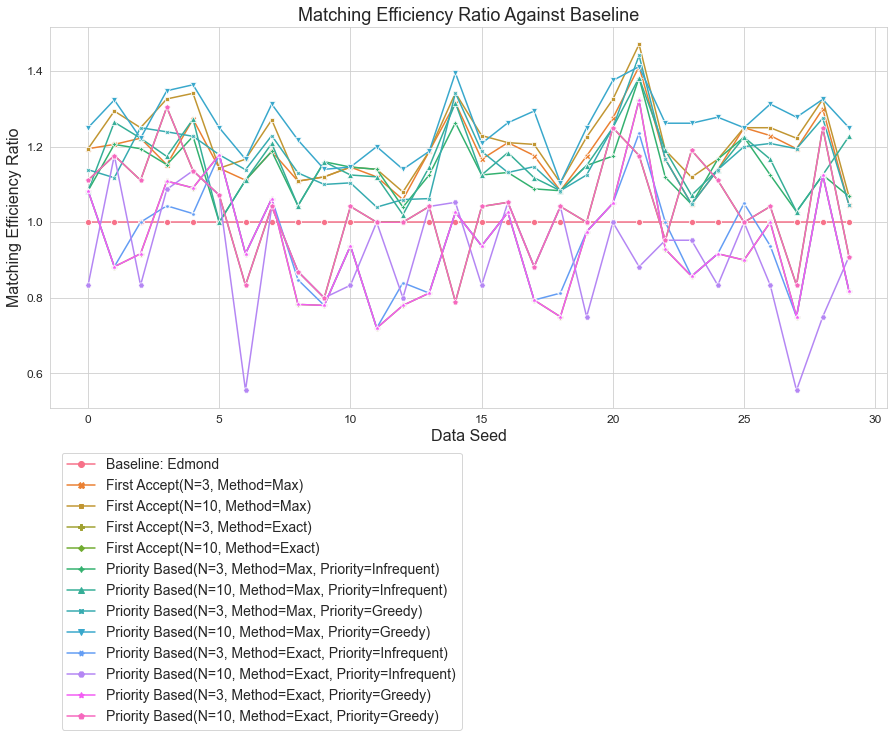
\includegraphics[width=0.5\textwidth]{images/matching_efficiency_ratio_against_baseline.png}
    \caption{Matching Efficiency Ratio of \textit{N}-way Algorithms against Baseline}
    \label{matcheffratio}
\end{figure}

To simplify the figure, Table \ref{tab2} is used to store average matching efficiency improvement ratio in compared to baseline. The average used
in the table is the average improvement ratio of an algorithm in comparison to baseline for all data seeds.

\begin{table}[htbp]
    \caption{Average Matching Efficiency Ratio of \textit{N}-way Algorithms compared to Baseline}
    \begin{center}
    \def\arraystretch{1.5}
    \begin{tabular}{|c|c|}
    \hline
    \cellcolor{tableheader}&\cellcolor{tableheader}\textbf{Average} \\
    \cellcolor{tableheader}\textbf{Algorithm}&\cellcolor{tableheader}\textbf{Improvement}\\
    \cellcolor{tableheader}&\cellcolor{tableheader}\textbf{Ratio}\\
    \hline
    Baseline: Edmond's Algorithm&1.0 \\
    \hline
    First Accept(N=3, Method=Max)&\cellcolor{moreratio}1.18 \\
    \hline
    First Accept(N=10, Method=Max)&\cellcolor{moreratio}1.22 \\
    \hline
    First Accept(N=3, Method=Exact)&\cellcolor{lessratio}0.94 \\
    \hline
    First Accept(N=10, Method=Exact)&\cellcolor{moreratio}1.04 \\
    \hline
    Priority Based(N=3, Method=Max, Priority=Greedy)&\cellcolor{moreratio}1.17 \\
    \hline
    Priority Based(N=10, Method=Max, Priority=Greedy)&\cellcolor{moreratio}1.26 \\
    \hline
    Priority Based(N=3, Method=Max, Priority=Infrequent)&\cellcolor{moreratio}1.14 \\
    \hline
    Priority Based(N=10, Method=Max, Priority=Infrequent)&\cellcolor{moreratio}1.16 \\
    \hline
    Priority Based(N=3, Method=Exact, Priority=Greedy)&\cellcolor{lessratio}0.94 \\
    \hline
    Priority Based(N=10, Method=Exact, Priority=Greedy)&\cellcolor{moreratio}1.04 \\
    \hline
    Priority Based(N=3, Method=Exact, Priority=Infrequent)&\cellcolor{lessratio}0.95 \\
    \hline
    Priority Based(N=10, Method=Exact, Priority=Infrequent)&\cellcolor{lessratio}0.91 \\
    \hline
    \end{tabular}
    \label{tab2}
    \end{center}
\end{table}

As can be seen from Table \ref{tab2}, most of \textit{N}-way match map searching algorithm produces higher matching efficiency in
comparison to the baseline, Edmond's Algorithm. However, some algorithms, using the exact method of using \textit{N} parameter,
have worse results compared to baseline. The average matching efficiency of the \textit{N}-way match map searching
algorithms is 7.75\% higher than the baseline algorithm. The higher matching efficiency improvement is obtained when First Accept
Searching algorithm is used when \textit{N} is 10, maximum method of using \textit{N}, with data seed 21, where the improvement
against baseline is 47.06\%.

While \textit{N}-way match map searching algorithms may produce better results, it is worth noting that with \textit{N}-way exchanges
being produced by algorithm may be harder to execute in hospitals since the kidney exchanges have to be operated in the same time. The
implication is that exchanges with lower number of ways are easier to conduct as less hospital resources are needed to conduct the operation.
Therefore, there needs to be an algorithm comparison regarding the average and the maximum exchanges length of the cycles in the match map.
In this experiment, every algorithm and parameter combinations are being tested for 30 data seeds with each containing 100 incompatible pairs. 

\begin{figure}[h]
   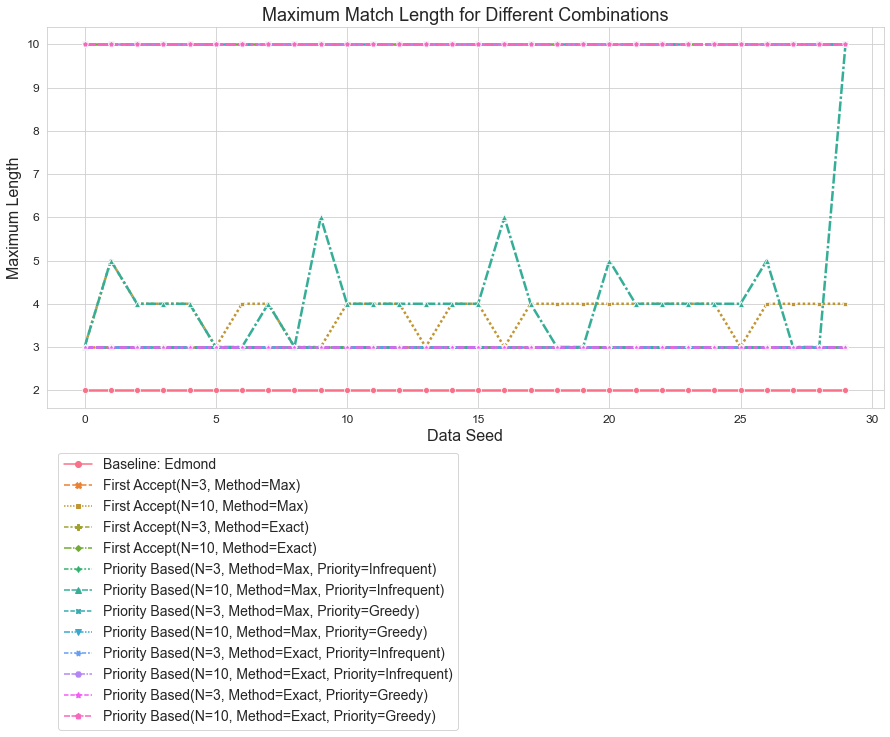
\includegraphics[width=0.5\textwidth]{images/maximum_match_length_for_different_combinations.png}
   \caption{Maximum Match Length for Different Algorithm Combinations}
   \label{figuremaxlength}
\end{figure}

From what can be seen in Figure \ref{figuremaxlength}, Edmond's Algorithm and algorithms with \textit{N} usage method parameter assigned to exact, produced the maximum
length of \textit{N} as the cycles in the produced match map is all of the same length that is \textit{N}.
The more interesting result is that although the parameter \textit{N} is 10, as can be seen with the green and the yellow line, the maximum length is
is not that close to 10. 

\begin{figure}[h]
    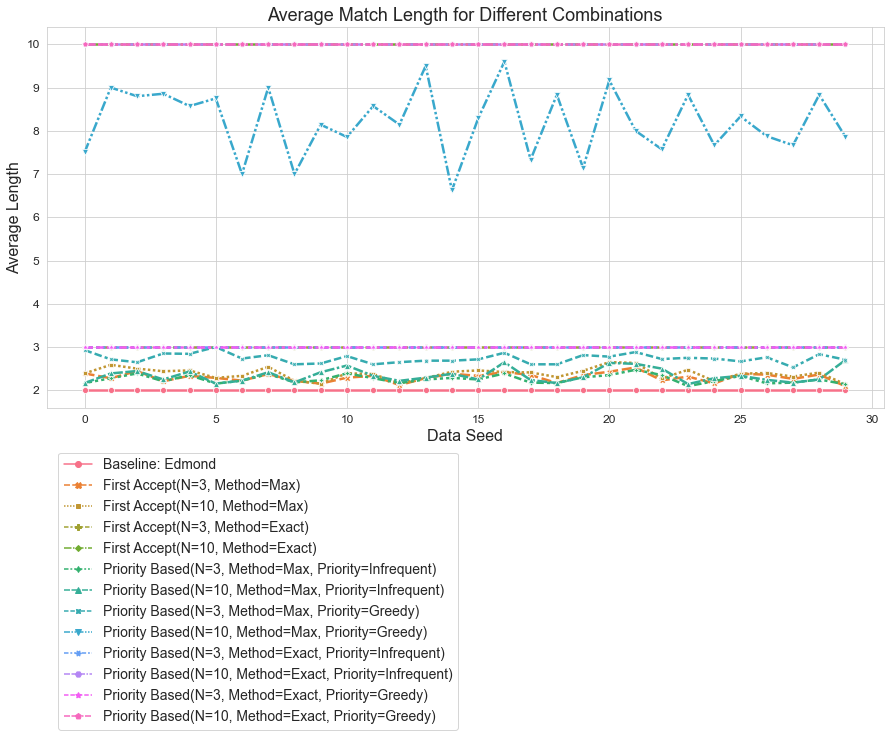
\includegraphics[width=0.5\textwidth]{images/average_match_length_for_different_combinations.png}
    \caption{Average Match Length for Different Algorithm Combinations}
    \label{figureavglength}
\end{figure}

Similar to what can be seen in Figure \ref{figuremaxlength}, in Figure \ref{figureavglength}, Edmond's Algorithm and algorithms with
\textit{N} usage method parameter assigned to exact, produced the average length of \textit{N} as the cycles in the produced match map is all
of the same length that is \textit{N}. Generally, almost every algorithm that uses maximum method of \textit{N} usage produces cycles with the
average length of around 2 to 3, with Priority-based Searching algorithm with N=10, Method=Max, and Priority=Greedy, having an averagely high
average length of exchanges.

\section{Conclusion}
This paper shows that it is a viable option to use \textit{N}-way match map searching algorithms instead of the usual two-way
algorithms such as Edmond's Algorithm for Kidney Paired Donation, with \textit{N}-way algorithms producing better matching efficiency
and competitive execution time in comparison to the baseline, Edmond's Algorithm provided the same dataset. Generally speaking,
the usage of \textit{N}-way algorithms increases matching efficiency by 7.75\%.

With the provided data, First Accept Searching algorithm have a more consistent performance in general compared to Priority-based Searching
algorithm. However, with Priority-based Searching algorithm, the matching efficiency improvement is generally higher with the exception of
when exact method to utilize \textit{N} is being used instead of the maximum method. However, it is worth noting that priority-based searching
algorithm may produce high matching efficiency with the compromise of high average matching length if greedy priority assignment method is being
used. Therefore it can be concluded that First Accept Searching algorithm is the most ideal \textit{N}-way match map searching algorithm to use
in Kidney Exchange Program. 

\section{Related Work}
The idea of the solution, the existing algorithms, and the performance metrics being used as a performance measure are all obtained from
the main reference paper, Web Based Decision Support System for Kidney Exchange by Samy Raja, Prasanna Devi S., and Suryaprakasa Rao K. in
International Journal of Computer Applications \cite{raja}. In that paper, two-way match map searching algorithms are being used to tackle
the problem of the humanely-impossible task of searching the most optimal match map out of an incompatible pairs pool, which becomes the baseline
and the reference of the newer algorithms being implemented in this paper.

\begin{thebibliography}{00}
\bibitem{roth2005} Roth, A. E., Sonmez, T., Unver, M. U. (2005). Kidney Exchange. Quarterly Journal of Economics, 32.
\bibitem{wiradarma} Wiradarma, K. (2016, February 3). Transplantasi Ginjal di Indonesia: Pencapaian dan Hambatannya. Retrieved from klikdokter.com: https://www.klikdokter.com/info-sehat/read/2697086/transplantasi-ginjal-di-indonesia-pencapaian-dan-hambatannya
\bibitem{roth2006} Roth, A. E., Sonmez, T., Unver, M. U., Delmonico, F. L., Saidman, S. L. (2006, September 18). Utilizing List Exchange and Nondirected Donation through ‘Chain’ Paired Kidney Donations. Retrieved from onlinelibrary.wiley.com: https://onlinelibrary.wiley.com/doi/full/10.1111/j.1600-6143.2006.01515.x
\bibitem{adrian} Adrian, K. (2020, May 17). Berbagai Persiapan Donor Ginjal yang Perlu Anda Ketahui. Retrieved from alodokter.com: https://www.alodokter.com/hal-hal-yang-harus-diperhatikan-sebelum-melakukan-donor-ginjal
\bibitem{raja} Raja, S., S., P. D., K., S. R. (2011). Web Based Decision Support System for Kidney. International Journal of Computer Applications (0975 – 8887), 9.
\bibitem{charge} Chargé, S., Hodgkinson, K. (2017, January). Blood: the basics. Retrieved from profedu.blood.ca/: https://profedu.blood.ca/en/transfusion/publications/blood-basics.
\bibitem{aprilano} Aprilano, W. D. (2021, January 20). Teknik Transplantasi Ginjal. Retrieved from alomedika.com: https://www.alomedika.com/tindakan-medis/transplantasi/transplantasi-ginjal/teknik
\bibitem{nguyen} Nguyen, H. D., Williams, R. L., Wong, G., Lim, W. H. (2013, February 13). The Evolution of HLA-Matching in Kidney Transplantation. Retrieved from intechopen.com: https://www.intechopen.com/books/current-issues-and-future-direction-in-kidney-transplantation/the-evolution-of-hla-matching-in-kidney-transplantation
\bibitem{tullis} Tullis, T., Albert, B. (2013, June 3). Performance Metrics. Retrieved from sciencedirect.com: https://www.sciencedirect.com/science/article/pii/B9780124157811000042
\bibitem{sedgewick} Sedgewick, R., Wayne, K. (2020). Directed Graphs. In R. Sedgewick, K. Wayne, Algorithms, 4th Edition (p. 955). New Jersey: Princeton University.
\bibitem{mehta} Mehta, D. (2020, May 27). Detect Cycle in a Directed Graph. Retrieved from geeksforgeeks.org: https://www.geeksforgeeks.org/detect-cycle-in-a-graph/
\end{thebibliography}

\end{document}
